\chapter{EXPERIMENTAL RESULTS AND DISCUSSION}
In this chapter, we will present a comprehensive analysis of the experimental results obtained from our implementation of the Spectral Transformation Lanczos algorithm for the symmetric definite generalized eigenvalue problem. We examine the algorithm performance on a test matrix, analyze the effects of ill-conditioning on convergence and accuracy, and compare the error bounds with what was predicted with direct methods.

\section{Software and Computational Environment}
The numerical experiments in this thesis are performed using the Python programming language together with the NumPy $2.0.2$ and SciPy $1.13.1$ libaries which makes function calls to optimized and efficient LAPACK and BLAS routines for linear algebra computations. These libraries ensure high-performance matrix operations and numerical stability. All computations are performed in \textbf{double precision} (64 bit floating point, \texttt{float64}) to maintain numerical accuracy and consistency.

For reproducibility, all code is written in Python $3.9.6$ and executed within a controlled environment using \texttt{virtualenv}. All numerical results have been validated by comparing different levels of precision where applicable and verifying consistency with analytical results when available. Code for the experiments is managed using version control with Git to ensure reproducibility and can be found in \href{https://github.com/AyobamiAdebesin/ayobami_thesis}{https://github.com/AyobamiAdebesin/ayobami\_thesis}

\section{Experimental Setup}
To evaluate the ST-Lanczos algorithm, we employ Algorithm (\ref{alg:problem_setup}) to generate test matrices $A$ and $B$ with controlled eigenvalue distribution. For the purpose of this thesis, we will be testing with dense matrices The eigenvalues are divided into 3 distinct groups, each with a specified range (spread). For each of the three groups, a random set of eigenvalues was generated using a uniform distribution, ensuring that the eigenvalues are distributed evenly within their respective ranges.

\begin{itemize}
    \item[$\bullet$] Group $1$ contains $1500$ eigenvalues in the range $(1, 199)$
    \item[$\bullet$] Group $2$ contains $400$ eigenvalues in the range $(200, 300)$
    \item[$\bullet$] Group $3$ contains $100$ eigenvalues in the range $(301, 400)$
\end{itemize}

The three sets of eigenvalues are then concatenated into a single array $D \in \mathbb{R}^{2000 \times 2000}$, which is then used with a regularization hyperparameter $\delta = 10^{-2}$, to generate $A$ and $B$ of size $2000 \times 2000$. Our shift is choosen to be $\sigma = 201$. For this choice of $\delta$, the condition number of $A$ and $B$ are as follows:
\begin{equation*}
    \kappa(A) = 1.23 \times 10^7, \qquad \kappa(B) = 5.39 \times 10^5
\end{equation*}
As discussed in section \ref{sec:ProblemSetup}, $A$ and $B$ will be symmetric with $B$ being positive definite. $B$ is factored using the SciPy \texttt{cholesky} method which calls LAPACK \textbf{\texttt{xPOTRF}}. We chose to use this since $B$ was designed to be strictly positive definite. We run Algorithm \ref{alg:spectral_lanczos_algorithm} for $n=1200$ iterations for the spectral problem
\begin{equation}\label{eq:ShiftedInvertedProblem2}
	C_b^T (A-\sigma B)^{-1} C_b \mathbf{u} = \theta \mathbf{u}, \qquad \mathbf{u} \neq \mathbf{0}
\end{equation}
to compute the lanczos decomposition using various decompositions techniques for $A - \sigma B$ that was discussed in section \ref{sec:SpectralTransformationDescription}. We explored these techniques and discuss the results in the following sections.

\section{Metrics}
To evaluate the efficiency of the ST-Lanczos algorithm, we define the following metrics

\begin{equation}\label{eq:DecompositionResidual}
\text{Relative Decomposition Residual} = \frac{\|BQ_n - Q_nT_n - \mathbf{q}\mathbf{x}^T\|}{\|B\|},
\end{equation}
where $B = C_b^T (A-\sigma B)^{-1} C_b $.

\begin{equation}\label{eq:GeneralizedResidual}
\text{Generalized Relative Residual} = \frac{\| (\beta A - \alpha B)\mathbf{v} \| }{(\lvert \beta \rvert \|A\| + \lvert \alpha \rvert \|B\|)\|v\| }
\end{equation}

\begin{equation}\label{eq:STResidual}
\text{ST Relative Residual} = \frac{\| C_b^T(A - \sigma B)^{-1}C_b \mathbf{u} - \lvert \theta \rvert \mathbf{u} \| }{( C_b^T(A - \sigma B)^{-1}C_b + \lvert \theta \rvert)\|\mathbf{u}\| }
\end{equation}

\section{$LU$ decomposition}
The $LU$ decomposition of $A - \sigma B$ is performed using the \texttt{linalg.lu\_factor} function in SciPy, which employs partial pivoting. For $n = 1200$ iterations, the Krylov solution subspace has a dimension of $1200$, and the ST Lanczos algorithm achieves a decomposition residual of the order of $10^{-10}$, despite a full reorthogonalization. This reduction in accuracy is attributed to pivot-limited accuracy. Using a tolerance of $10^{-10}$ for the Ritz pair residuals computed by (\ref{eq:STResidual}), approximately $75\%$ of the Ritz pairs converge with an accuracy of the order $10^{-13}$ for Ritz values close to the shift. However, the generalized residuals for these converged Ritz pairs remain on the order of machine precision $u=10^{-16}$. As shown in Fig \ref{fig:LUResidualsIll}, the residuals are small for eigenvalues near the shift and gradually tends to increase for larger eigenvalues, consistent with the error bounds proven by (Michael Stewart, 2024) for a direct method. To examine the effect of conditioning, $\delta$ was increased to $\delta=10^2$ so that $\kappa(A) = 4013$ and $\kappa(B) = 54.9$. For this \textit{well-conditioned} problem, the Lanczos decomposition residual decreases to the order of $10^{-13}$, indicating that the accuracy of the Lanczos decomposition is influenced by the problem's conditioning. Additionally, for the same tolerance, an improvement in the Ritz pair residuals was observed  while the generalized residuals was not impacted by the problem's conditioning as shown in Fig \ref{fig:LUResidualsWell}.

\begin{figure}
\centering
        \caption{Residuals plot for ill-conditioned problem}
	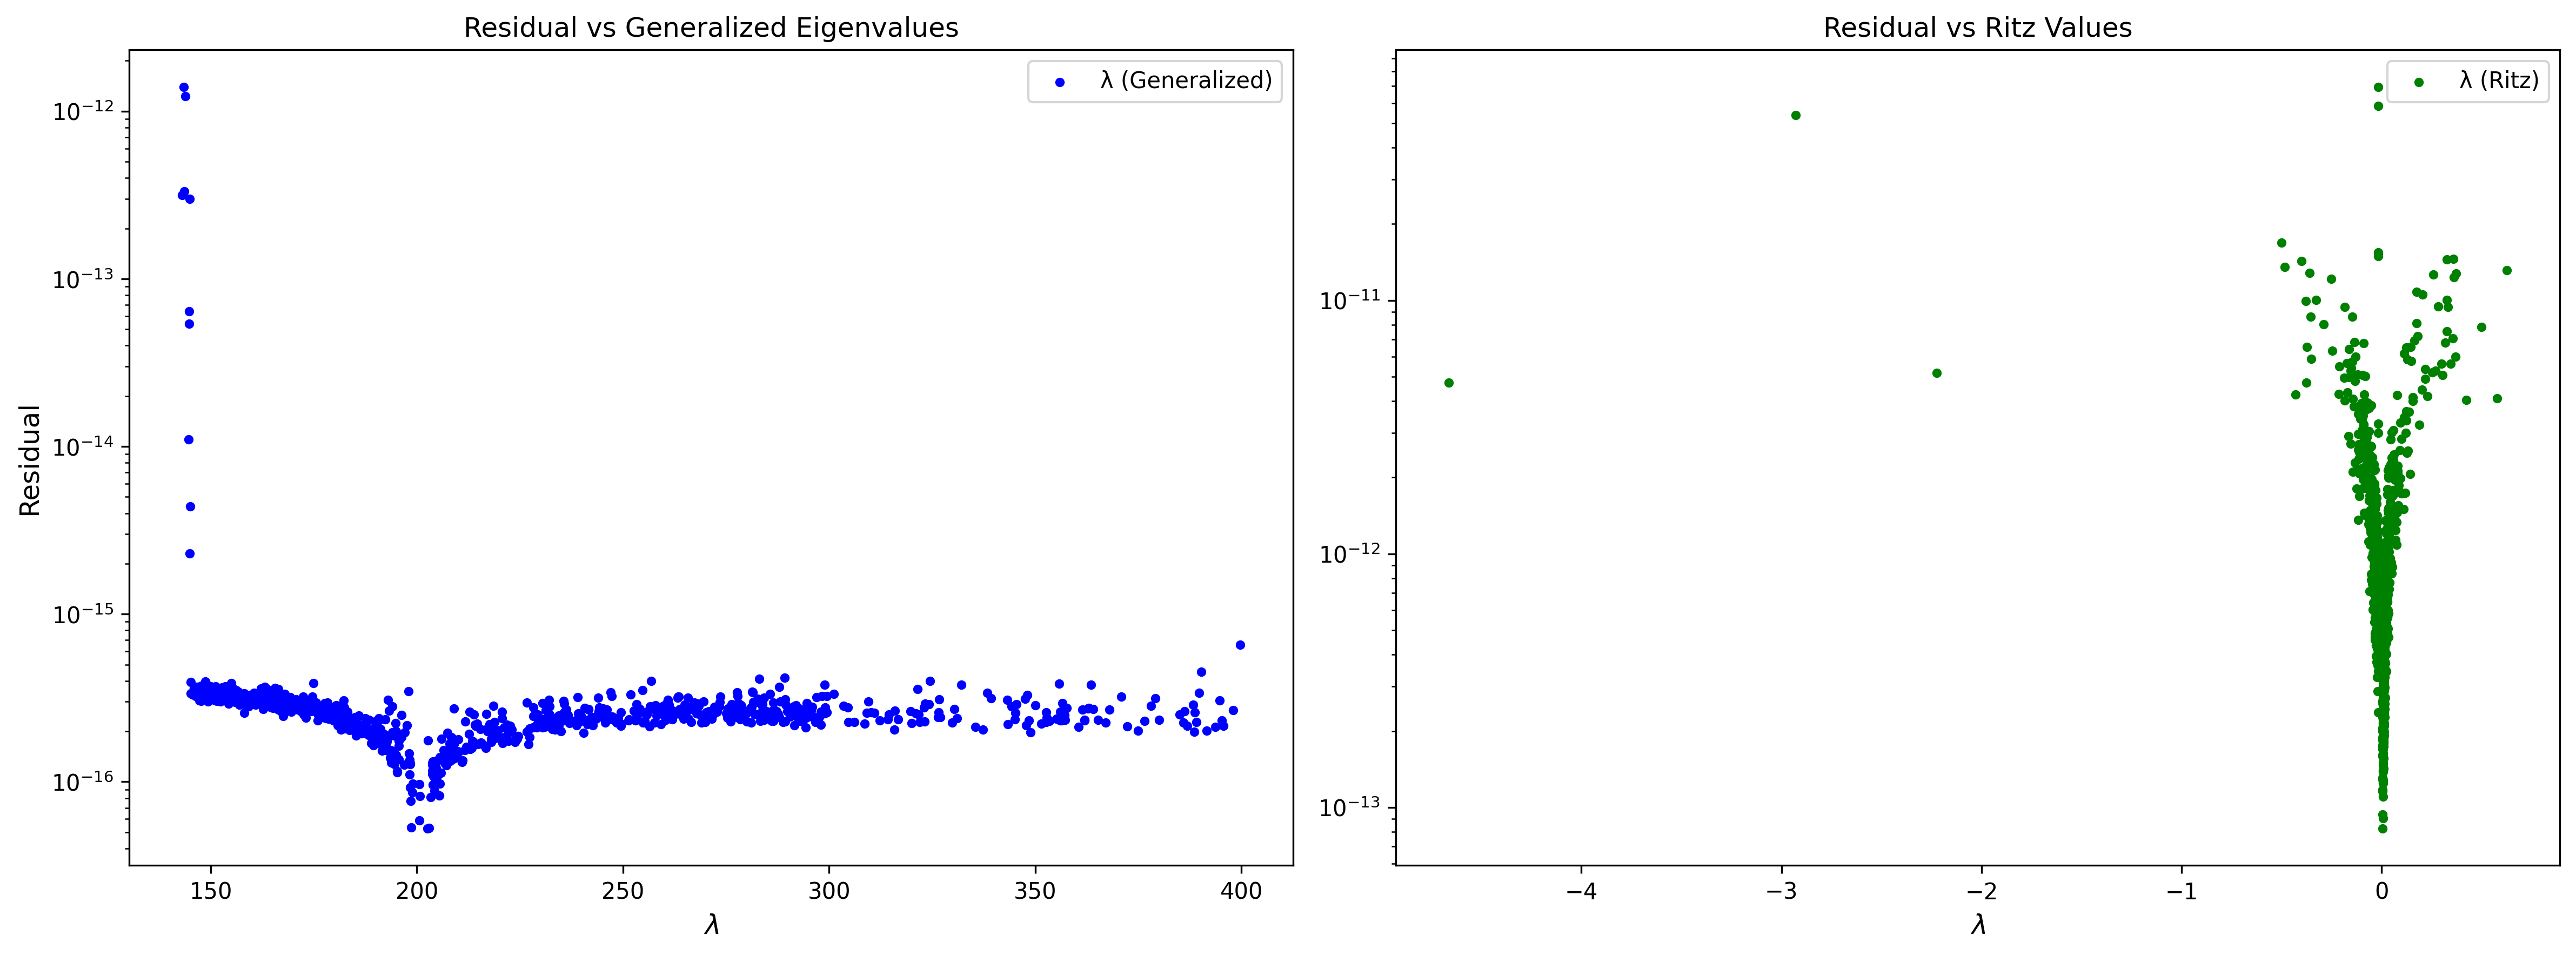
\includegraphics[height=2.5in]{./Plots/LU/residuals_plot_ill.png}
	
        \label{fig:LUResidualsIll}
\end{figure}

\begin{figure}
\centering
        \caption{Residuals plot for well-conditioned problem}
	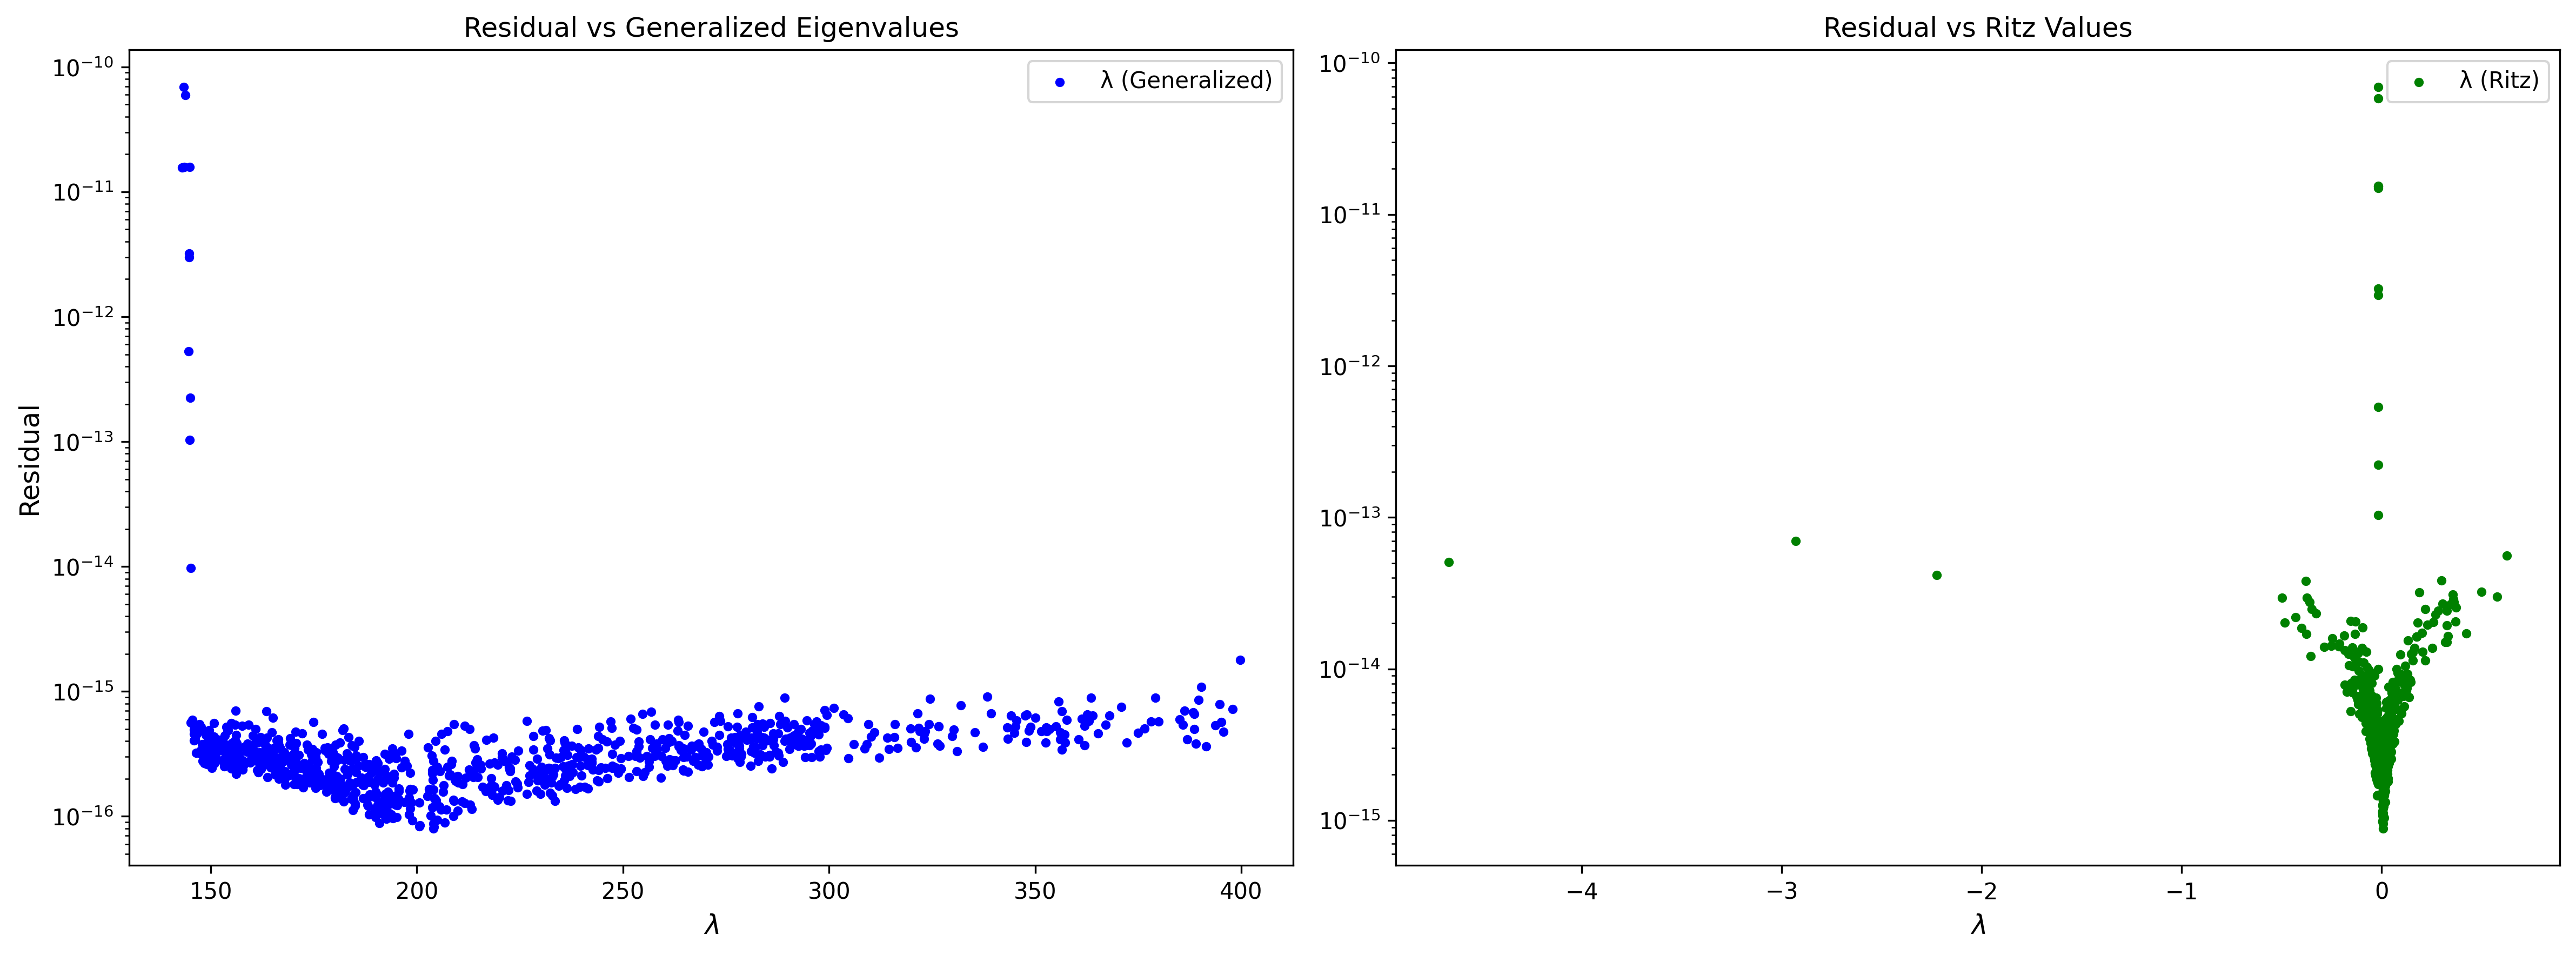
\includegraphics[height=2.5in]{./Plots/LU/residuals_plot_well.png}
	
        \label{fig:LUResidualsWell}
\end{figure}

\section{Eigenvalue Decomposition}
Another decomposition technique we employed is the symmetric eigenvalue decomposition of $A-\sigma B$ given by
\begin{equation}
    A-\sigma B = WDW^T,
\end{equation}
so that the spectral transformed problem is given by
\begin{equation}\label{3.4}
	C_b^T W^{-T}D^{-1}W^{-1} C_b \mathbf{u} = \theta \mathbf{u}, \qquad \mathbf{u} \neq \mathbf{0}
\end{equation}
This decomposition, done using \texttt{linalg.eigh} function in SciPy, uses the LAPACK \texttt{dsyevd} routine for real symmetric matrices, which in turn uses divide-and-conquer algorithms for efficiency. The Lanczos decomposition residual was observed to be of the order $10^{-23}$, indicating a highly accurate decomposition. The results of the residual analysis are presented in Fig \ref{fig:EigDecompRes}
On the left plot, the residuals remain on the order of machine precision $10^{-17}$ for most eigenvalues. Similarly, on the right of the plot, the Ritz residuals are minimized near $\theta = 0$ with values on the order of machine precision and gradually increasing for larger Ritz values. To assess the effect of ill-conditioning, $\delta$ was reduced to $\delta = 10^{-5}$, so that $\kappa(A) = 8.2 \times 10^9$ and $\kappa(B) = 5.4 \times 10^8$. It was observed that this ill-conditioning did not affect the computed residuals with.\\
Overall, the extremely low decomposition residual confirms the robustness of using a decomposition that preserves symmetry, while the observed trends in residuals highlight the sensitivity of numerical accuracy to the spectrum of the problem.

\begin{figure}
\centering
        \caption{Residuals plot for $A -\sigma B = WDW^T$}
	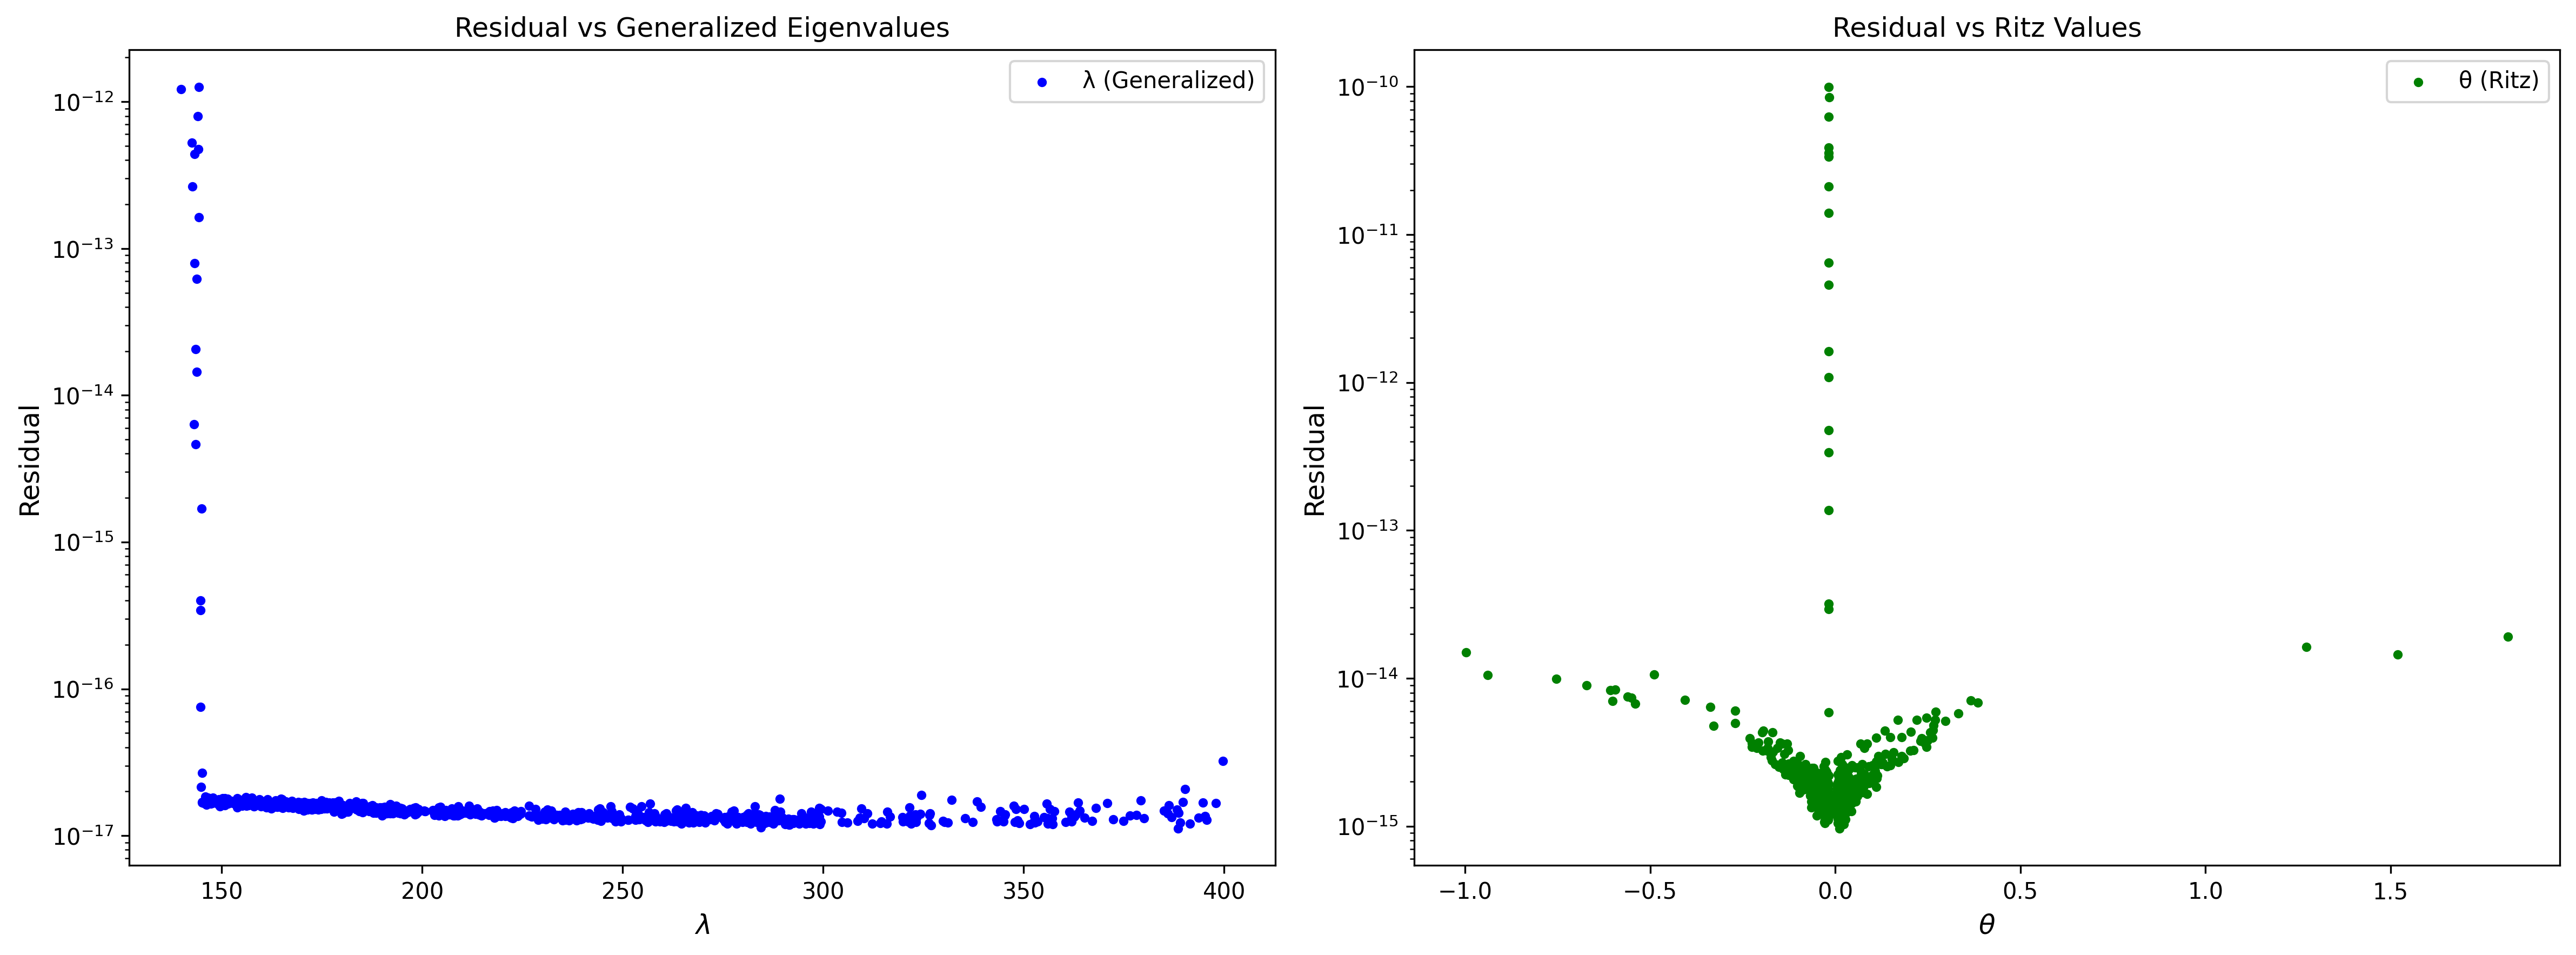
\includegraphics[height=2.5in]{./Plots/eigdecomp/eig_residual_plots.png}
        \label{fig:EigDecompRes}
\end{figure}